\documentclass[a4paper,12pt]{article}

%%% Работа с русским языком
\usepackage{cmap}					% поиск в PDF
\usepackage{mathtext} 				% русские буквы в формулах
\usepackage[T2A]{fontenc}			% кодировка
\usepackage[utf8]{inputenc}			% кодировка исходного текста
\usepackage[english,russian]{babel}	% локализация и переносы
\usepackage{xcolor}
\usepackage{hyperref}
 % Цвета для гиперссылок
\definecolor{linkcolor}{HTML}{00FFFF} % цвет ссылок
\definecolor{urlcolor}{HTML}{4682B4} % цвет гиперссылок

\hypersetup{pdfstartview=FitH,  linkcolor=linkcolor,urlcolor=urlcolor, colorlinks=true}

%%% Дополнительная работа с математикой
\usepackage{amsfonts,amssymb,amsthm,mathtools} % AMS
\usepackage{amsmath}
\usepackage{icomma} % "Умная" запятая: $0,2$ --- число, $0, 2$ --- перечисление

%% Номера формул
%\mathtoolsset{showonlyrefs=true} % Показывать номера только у тех формул, на которые есть \eqref{} в тексте.

%% Шрифты
\usepackage{euscript}	 % Шрифт Евклид
\usepackage{mathrsfs} % Красивый матшрифт

%% Свои команды
\DeclareMathOperator{\sgn}{\mathop{sgn}}

\usepackage{enumerate}
%% Перенос знаков в формулах (по Львовскому)
\newcommand*{\hm}[1]{#1\nobreak\discretionary{}
{\hbox{$\mathsurround=0pt #1$}}{}}
% графика
\usepackage{graphicx}
\graphicspath{{picture/}}
\DeclareGraphicsExtensions{.pdf,.png,.jpg}
\author{Бурмашев Григорий, 208. \href{https://teleg.run/burmashev}{@burmashev}}
\title{Дискретная математика. Коллок -- 1. Определения и задачи по ним.}
\date{}
\begin{document}
\begin{center}
Бурмашев Григорий. Дискра -- 10
\end{center}
\subsection*{Номер 2}
Пусть у нас множества A и B -- это множество натуральных чисел (1, 2, 3, $\ldots$) заданы такие функции f и g:
\[
f: x \rightarrow x + 1
\]
\[
g:x \rightarrow x - 1
\]
Функция g не определена в точке x = 1, т.к переводит нас в 0, что выходит за рамки натуральных чисел. При этом все еще $g \circ  f = id$
\begin{center}
\textbf{Ответ:} нет, неверно 
\end{center}

\subsection*{Номер 3}
Наша функция f $x_1$ переводит в $x_2$, а $x_2$ переводит в $x_1$. А значит у нас образуются пары (чтобы получилась $id$). А значит элементов, которые переходят сами в себя, может быть 1, 3, 5 или все 7 (чтобы была возможность оставшимся образовать пары).
Рассмотрим все возможные случаи:
\begin{itemize}
\item  Если 1 элемент неподвижен:

Тогда оставшиеся 6 элементов образуют пары, подсчитаем все возможные случаи:
\[
\frac{\frac{6 \cdot 5}{2} \cdot \frac{4\cdot3}{2} \cdot \frac{2\cdot1}{2}}{3!} = 15 
\]
Итого:
\[
15 \cdot 7 = 105
\]
\item Если 3 элемента неподвижны:

Тогда оставшиеся 4 элемента разбиваются на пары:
\[
C_7^3 \cdot 3 = \frac{7!}{3!4!}  \cdot 3 = 35 \cdot 3 = 105
\]
\item Если 5 элементов неподвижны:

Тогда оставшиеся 2 элемента разбиваются на пары:
\[
C_7^5 \cdot 1 = 7 \cdot 3 = 21
\]
\item Если у нас все 7 элементов неподвижны:

Тогда всего 1 возможный случай.

В таком случае итого:
\[
105 + 105 + 21 + 1 = 232
\]
\end{itemize}
\begin{center}
\textbf{Ответ:} 232 варианта
\end{center}
\subsection*{Номер 4}
Можно привести пример:
\begin{center}
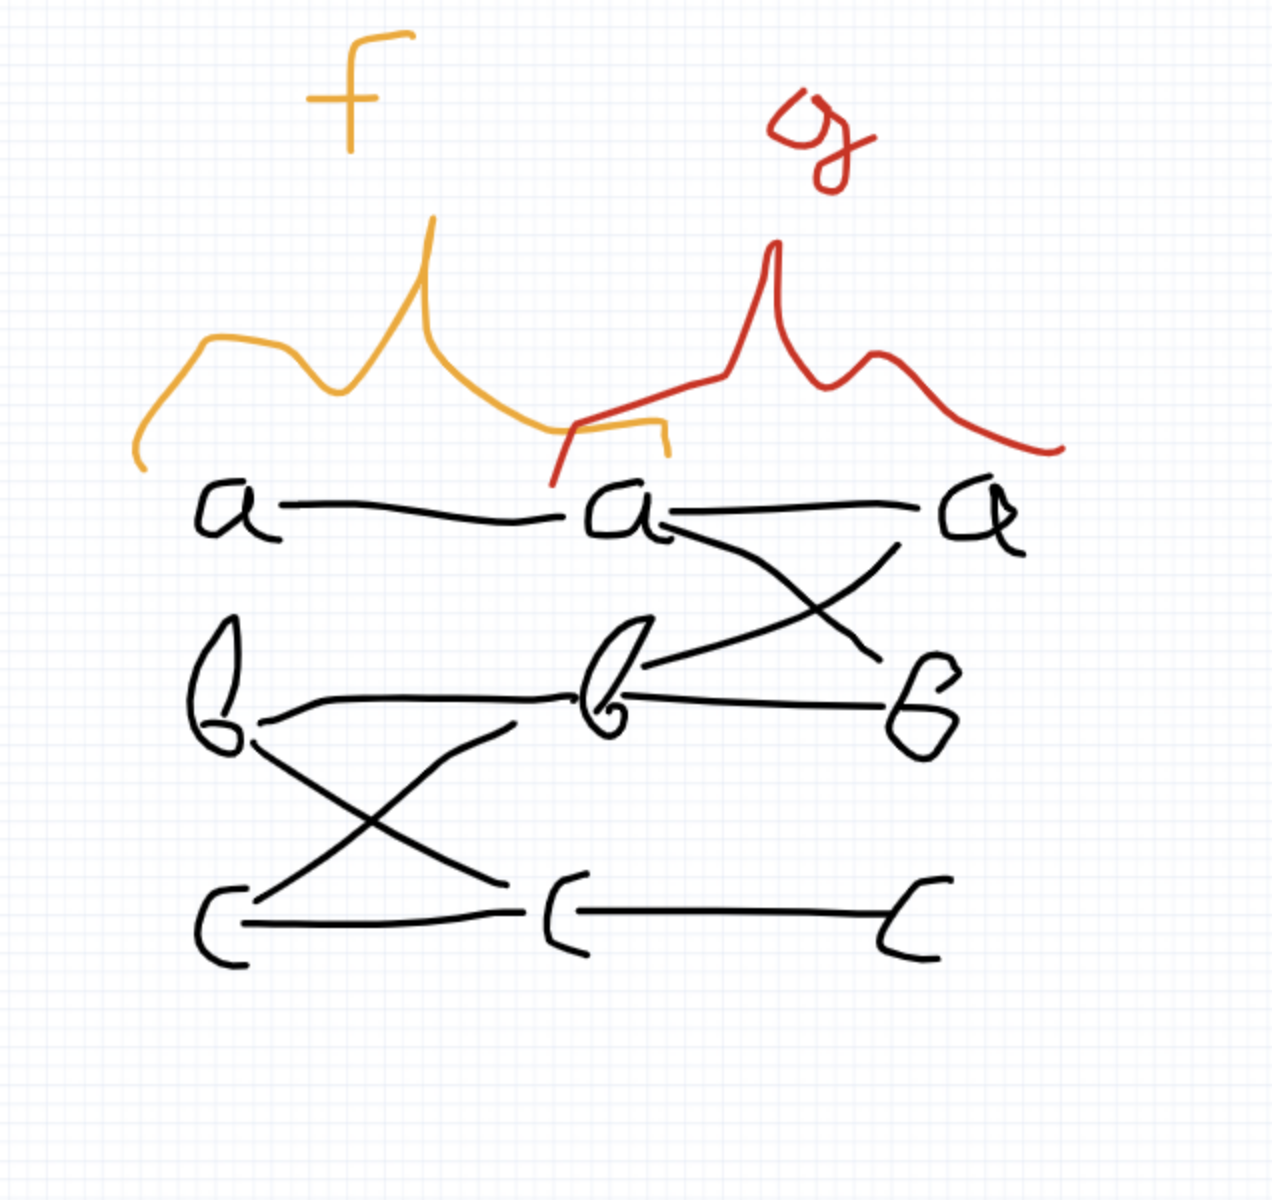
\includegraphics[scale=0.2]{abc.png}
\end{center}
Рассмотрим f:
\begin{equation*}
\begin{gathered}
a \sim a\\ b \sim c \\ c \sim b\\ b \sim b \\ c \sim c
\end{gathered}
\end{equation*}
Рассмотрим g:
\begin{equation*}
\begin{gathered}
a \sim a \\ 
a \sim b \\
b \sim a \\
b \sim b\\ 
c \sim c\\
\end{gathered}
\end{equation*}
Значит f и g -- отношения эквивалентности. 

При этом в композиции (это видно на рисунке):

$c \sim a$. Но $a \nsim c$. А значит композиция отношений эквивалентности не всегда есть отношение эквивалентности.
\begin{center}
\textbf{Ответ:} нет
\end{center}
\subsection*{Номер 5}
У нас множество $\{1,  2, 3, 4 \}$. Переберем все возможные случаи, чтобы сохранялось отношение эквивалентности.
\begin{itemize}
\item 
Нет пар (биекция $a \sim a \; \forall a \in \{1, 2, 3, 4\}$)

Всего 1 единственный случай
\item
1 пара эквивалентности ($a \sim b$).

Ее можно выбрать:
\[
\frac{4 \cdot 3}{2}  =6 \text{ способами}
\]
\item
2 пары эквивалентности, которые не пересекаются ($a \sim b, a' \sim b '$).

Их можно выбрать:
\[
\frac{4 \cdot 3}{2} = 6 \text{ способами}
\]
\item
3 пары эквивалентности, но с пересечениями (например $ a \sim b, b \sim c, c \sim a$)

Их всего у нас:
\[
4 \cdot 3 = 12 \text{ способами}
\]
\item
Если все эквивалентны друг другу:

Всего 1 единственный случай

\item
Итого:
\[
1 + 6 + 6 + 12 + 1 = 26
\]
\end{itemize}
\begin{center}
\textbf{Ответ:} 26
\end{center}
\subsection*{Номер 6}
\textbf{a)}
По определению симметричности:

если $a \sim b$,  то $b \sim a$. Очевидно, что у нас должно быть четное число таких пар (иначе какого-то $b \sim a$ будет не хватать). Но у нас 33 пары. А поскольку 33 нечетно, то такого быть не может
\begin{center}
\textbf{Ответ:} нет
\end{center}


\subsection*{Номер 7}
\textbf{a)} У чисел x и y одинаковая последняя цифра.

Проверяем условия отношения эквивалентности:

1) $a \sim a$ очевидно (a и a заканчиваются на одно и тоже число a')

2) Пусть число a заканчивается на $a'$, а число b  заканчивается на $b'$. Если $a \sim b$. Из этого автоматически следует, что $a' = b'$. А значит $b \sim a$.

3) Пусть число a заканчивается на $a'$,  число b  заканчивается на $b'$, а число c заканчивается на $c'$. Если $a \sim b$, то $a' = b'$. А если при этом $b \sim c$, то значит $b' = c'$. Ну а отсюда мы тогда получаем, что $a' = c'$ и $a \sim c$.
\begin{center}
\textbf{Ответ: } да
\end{center}
\textbf{б)} Числа x и y отличаются ровно в одном месте.

Можно привести контрпример:

Пусть есть числа a = 12 и b = 13. Они различатся ровно в одном месте (2 и 3). А значит $a \sim b$. Введем еще одно число c = 43. Оно отличается от b ровно в одном месте (1 и 4), т.е $b \sim c$. Но при этом a отличается от c в обоих позициях, т.е $a \nsim c$. А значит транзитивность не выполнена и они не являются отношениями эквивалентности.
\begin{center}
\textbf{Ответ: } нет
\end{center}

\textbf{в)} Разность между суммами цифр чисел x  и y четна.

Проверяем услвоия отношения эквивалентности:

1) Разность суммы чисел двух одинаковых цифр равна нулю (a - a = 0), значит $ a \sim a$

2) Разность суммы чисел двух цифр в любом порядке по модулю одинакова (|a - b| = |b - a|), значит $a \sim b \rightarrow b \sim a$.

3) Пусть есть три числа a, b и c. Пусть разность a - b = 2x. А разность b - c = 2x'. Т.е $a \sim b$ и $b \sim c$.  Тогда a - c = a - b + b - c = 2x - 2x' = 2(x - x'). Это тоже является четным числом, а значит $a \sim c$.

\begin{center}
\textbf{Ответ: } да
\end{center}
\subsection*{Номер 8}
Рассмотрим всевозможные случаи удаления ребер:
\begin{itemize}
\item
Пусть мы удалили ребро между вершинами степеней 3 и 4. Тогда у нас появилась 1 вершина степени 2 и 1 новая вершина степени 4. Но вершин степени 2 у нас вообще не было $\rightarrow$ изоморфности не будет

\item 
Пусть мы удалили ребро между вершинами степени 3. Тогда у нас останется 8 - 2 = 6 вершин степени три. И в каждой из компонент связности будет по 3 вершины степени три. Ну а значит сумма степеней вершин будет нечетна и изоморфности не будет.
\item 
Пусть мы удалили ребро между вершинами степени 4. Тогда у нас будет 8 + 2 = 10 вершин степени три. И в каждой из компонент связности будет по 5 вершин степени три. Ну а значит сумма степеней вершин будет  нечетна и изомфорности не будет

Других случаев удаления ребер у нас нет.
\begin{center}
\textbf{Ответ:} Ч.Т.Д
\end{center}
\end{itemize}
\end{document}